\documentclass{article}
\usepackage[utf8]{inputenc}
\usepackage{polski}
\usepackage[polish]{babel}
\usepackage{graphicx}    
\usepackage{caption}
\usepackage{subcaption}
\usepackage{epstopdf}
\usepackage{amsmath}
\usepackage{amsthm}
\usepackage{hyperref}
\usepackage{url}
\usepackage{comment}
\newtheorem{defi}{Definicja}
\newtheorem{twr}{Twierdzenie}
\setlength{\parindent}{0pt}


\author{Kacper Kulczak 279079}
\date{Wrocław, \today}
\title{\textbf{Odtwarzanie w przybliżeniu zadanej linii } \\ Sprawozdanie do zadania P.2.12}

\begin{document}
\maketitle

\section{Wstęp}

Wybrane przeze mnie zadanie polega na odtworzeniu w przybliżeniu linii przechodzącej przez zadane punkty $(x_1,y_1),(x_2,y_2),\dots,(x_n,y_n)$. Będziemy stosować do tego celu interpolację.\\

W paragrafie \S 2 przedstawiono sposoby na sprowadzenie problemu przybliżenia zadanej linii, do problemu interpolacji paru funkcji. W paragrafie \S3, znajdują się metody interpolacji użyte w tym sprawozdaniu oraz ich implementacja. Testy i przykłady znajdują się w paragrafie \S4, a wnioski w paragrafie \S5.\\

Wszystkie obliczenia były wykonywane  z wykorzystaniem języka programowania \textbf{Julia}, w pliku "program.jl". Wykresy zostały narysowane przy pomocy biblioteki \textbf{Plotly} w pliku "program.ipynb".



\section{Metody odtwarzania linii}
W celu odtworzenia linii skorzystam z dwóch następujących metod:
\begin{enumerate}
	\item \label{podzialFunkcji}Spróbujmy podzielić zadany ciąg punktów, na takie podciągi, żeby każdy zawierał punkty leżące na wykresie pewnej funkcji. Następnie zinterpolujmy  każdą z tych funkcji i narysujmy wszystkie w jednym układzie współrzędnych.
	
	\item \label{Parameryczna} Potraktujmy linię jako krzywą parametryczną. Niech każdy punkt będzie się równał $(x(t),y(t))$, gdzie t jest parametrem przebiegającym zadany przedział. Zinterpolujemy funkcje $x(t), y(t)$, a następnie narysujemy tą krzywą parametryczną.
\end{enumerate}

Metoda \ref{podzialFunkcji} ma parę wad. Po pierwsze nie da się odtworzyć pionowej linii, jest to poważne ograniczenie. Po drugie ręczne dzielenie punktów na podciągi może być bardzo pracochłonne, dla dużych danych wręcz niemożliwe. Metoda \ref{Parameryczna} jest wolna od tych problemów.

\section{Metody użyte do interpolowania funkcji}


\subsection{Wzór interpolacyjny Newtona}

Podstawową metodą interpolacji, jest przybliżenie zadanej funkcji wielomianem posiadającym te same wartości w węzłach. Można taki wielomian n-tego stopnia znaleźć za pomocą wzoru interpolacyjnego Newtona.\cite{kincaid}

\begin{equation}\label{Newton}
p_{n}(x) = \sum_{k=0}^{n}f[x_{0},x_{1},\dots,x_{k}]\prod\limits_{j=0}^{k-1}(x-x_{j})
\end{equation}

Gdzie $x_0,x_1,\dots,x_n$ to węzły wielomianu, a $f[x_{0},x_{1},\dots,x_{k}]$ to ilorazy różnicowe. 

	\subsubsection{Implementacja}
	
	Do efektywnego wyznaczenia odpowiedniego wielomianu interpolacyjnego Newtona, przy zadanych $x_0,x_1,\dots,x_n,y_0,y_1,\dots,y_n$ potrzebujemy jedynie wyznaczyć odpowiednie ilorazy różnicowe. Potrzebujemy do tego następującego twierdzenia \ref{ilorazy roznicowe}.
	
		\begin{twr}
			\label{ilorazy roznicowe}
			Ilorazy różnicowe spełniają zależności:
			$$f[x_k] = f(x_k)$$
			\begin{equation}
			f[x_{0},x_{1},\dots,x_{k}] = \frac{f[x_{1},x_{2},\dots,x_{k}] - f[x_{0},x_{1},\dots,x_{k-1}]}{x_k-x_0}
			\end{equation}
		\end{twr}
		\begin{proof}
			Udowodnione w \cite{kincaid} str 312
		\end{proof}
		
	Na podstawie powyższej własności, można zaimplementować poniższy algorytm. Znajduje się on również w \cite{kincaid}. Po zakończeniu algorytmu d[k] to iloraz $f[x_0,x_1,\dots,x_k]$ dla $(k=0,1,\dots,n)$
	
	\begin{verbatim}
	for i = 0 to n
	  d[i] := y[i]
	done
	for j=1 to n
	  for i=n to j
	    d[i] := (d[i] - d[i-1])/(x[i]-x[i-j])	
	  done
	done	
	\end{verbatim}
	
	Posiadając wyliczone ilorazy różnicowe, możemy prostą pętlą wyznaczyć odpowiedni wielomian interpolacyjny za pomocą wzoru \eqref{Newton}. 
	\\\\
	Interpolacja wzorem interpolacyjnym Newtona została zaimplementowana w pliku "interps.jl" dołączonym do sprawozdania.

\subsection{Naturalna funkcja sklejana III stopnia}
	
	Zamiast przybliżać funkcję, jedną zadaną funkcją, spróbujmy podzielić ją na kawałki i zinterpolujmy te kawałki. Tą idee wykorzystują funkcje sklejane, przybliżając kawałki wielomianami st. co najwyżej trzeciego.
	
	W źródle \cite{SLE} znajduje się definicja \ref{Def:Naturalna sklejana}, z której skorzystamy.
	
	\begin{defi}
		\label{Def:Naturalna sklejana}
		Dla danej liczby naturalnej $n$, danych węzłów $x_0,x_1,\dots,x_n \quad(a=x_0 < x_1 < \dots <$ $x_n = b)$ i danej funkcji $f$ naturalną funkcją sklejaną interpolującą III stopnia nazywamy $s$, określoną w przedziale $[a,b]$ i spełniającą następujące warunki:
	
		\begin{enumerate}
			\item $s, s', s''$ są ciągłe w $[a,b]$
			\item w każdym z przedziałów $[x_{k-1},x_k]$ \quad $(k=1,2,\dots,n) $ 
			\\
			funkcja $s$ jest wielomianem stopnia co najwyżej trzeciego
			\item $s(x_k)=f(x_k)$\quad $ (k = 0,1,\dots,n)$ 
			\item $s''(a) = s''(b) = 0$
		\end{enumerate}
	\end{defi}
	
	Więcej o funkcjach sklejanych można przeczytać w \cite{kincaid}.
	
	\subsubsection{Implementacja}
	
	W książce \cite{kincaid} pokazano, że naturalna funkcja sklejana III stopnia wyraża się wzorem: 
	\begin{multline}\label{Wzor: Sklejana}	
	 s_k(x) =  \frac{1}{6h_k}M_{k-1}(x_k-x)^3+\frac{1}{6h_k}M_k(x-x_{k-1})^3) + \\ \left(\frac{y_{k-1}}{h_k}-\frac{1}{6} M_{k-1}h_k \right)(x_k - x) + \left( \frac{y_k}{h_k}-\frac{1}{6} M_{k}h_k\right)(x-x_{k-1}) 
	\end{multline}
	
	Gdzie $M_k=s''x_k$,\quad $h_k=x_k-x_{k-1}$, \quad$(k=1,2,\dots,n)$\\
	
	Do zastosowania wzoru \eqref{Wzor: Sklejana} potrzebujemy obliczyć współczynniki $M_k$, będące drugą pochodną funkcji sklejanej w węzłach interpolacji. Wyznacza się je z następującego układu równań \eqref{Wzor: Uklad Sklejana}:
	
	\begin{equation}\label{Wzor: Uklad Sklejana}
	\lambda_kM_{k-1} + 2M_k + (1-\lambda_k)M_{k+1} = 6f[x_{k-1},x_k,x_{k+1}] \qquad (k=1,2,\dots,n-1)
	\end{equation}
	
	gdzie $\lambda_k = \frac{h_k}{h_k-h_{k+1}}$,\quad $h_k=x_k-x_{k-1}$
	\\\\
	Układ równań \ref{Wzor: Uklad Sklejana} można rozwiązać, za pomocą algorytmu podanego w \cite{SLE}:
	
	\begin{verbatim} 
	q[0] := u[0] := 0
	for k=1,2,...,n-1
	  p[k]=lambda[k]*q[k-1]+2
	  q[k]=(lambda[k-1])/p[k]
	  u[k]= (6f[x[k-1],x[k],[k+1]]-lambda[k]*u[k-1])/p[k]
	done
	M[n-1] = u[n-1]
	for k=n-2,n-3,...,1
	  M[k] := u[k] +q[k]*M[k]+1
	done
	\end{verbatim}
	
	Warto zauważyć, że przy interpolowaniu dwóch funkcji jednocześnie ($fx$ oraz $fy$ w węzłach $t_1,t_2,\dots,t_n$) dla krzywej parametrycznej , można zastosować te same $p_k,q_k$, ponieważ zależą one wyłącznie od $t_i$. Usprawni to wyliczenie współczynników $M_k$
	\\\\
	Naturalna funkcja sklejana III stopnia została zaimplementowana w pliku "interps.jl" dołączonym do sprawozdania.
	
\section{Przykłady}
	
	Wszystkie przykłady zostały zaprogramowane w języku \textbf{julia} w arytmetyce double. Funkcje interpolujące i obsługujące można znaleźć w pliku "program.jl", natomiast wykresy znajdują się w pliku "program.ipnyb" i zostały wygenerowane w bibliotece \textbf{Plotly}.

\subsection{Obrazki przybliżane zbiorem funkcji interpolowanych}	
	
	Linią, którą chciałbym przybliżyć, jest kontur ryby \ref{Ryba}.
	Ręcznie wyznaczono punkty z przedstawionego obrazka i przepisano je do programu. Punkty te zostały zaznaczone na wykresach.
	
		\begin{figure}[h]
			\centering
			
\includegraphics[width=0.2\textwidth]{rybka.jpg}
			\caption{Rysunek, który będziemy starać się przybliżyć}
			\label{Ryba}
		\end{figure}
		
	\subsubsection{Interpolacja wzorem Newtona}
	
	Najpierw skorzystamy z metody \ref{podzialFunkcji}. Wykres \ref{Wykres:Ryba_Newton} przedstawia uzyskane przez nas wyniki interpolacją wzorem Netwona.	
	
		\begin{figure}[h]
			\centering
			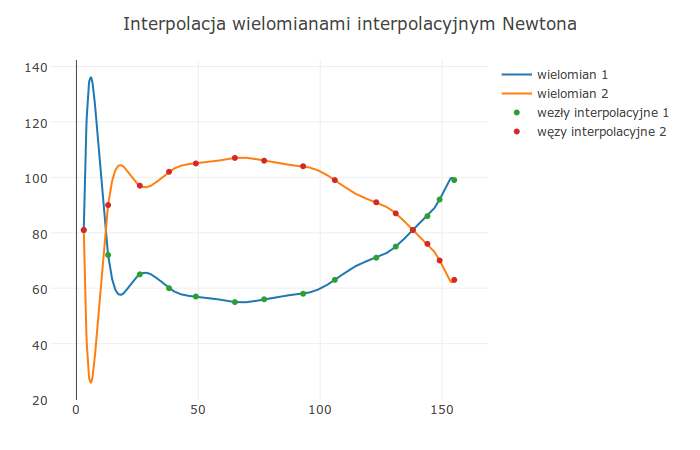
\includegraphics[width=0.8\textwidth]{newplot.png}
			\caption{Wykres przedstawiający rybę interpolowaną wielomianami Newtona.}
			\label{Wykres:Ryba_Newton}
		\end{figure}
		
	\newpage
	
	Widzimy, że nie daje to pożądanych efektów. Wielomiany interpolujące wyższego stopnia, potrafią mieć duże błędy na krańcach przedziałów. Dlatego w dalszej części sprawozdania, porzucimy interpolacje wzorem Newtona i skupimy się tylko na funkcjach sklejanych.
	
	\subsubsection{Interpolacja naturalną funkcją sklejaną}
	
	Na wykresie \ref{Wykres:Ryba_Sklejane} widnieje ryba, interpolowana dwoma naturalnymi funkcjami sklejanymi III stopnia.
	
		\begin{figure}[h]
			\centering
			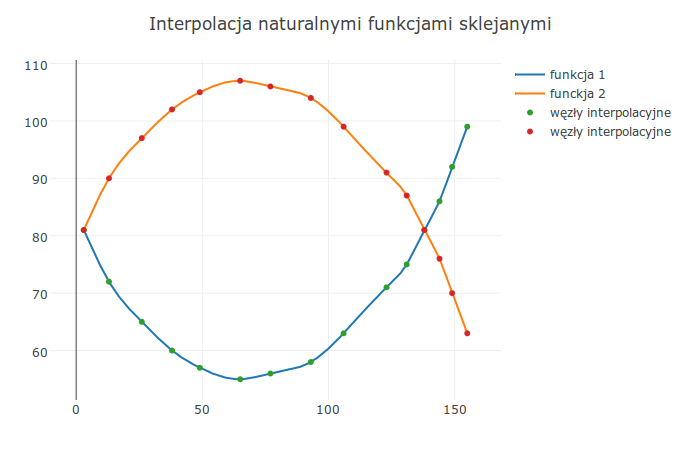
\includegraphics[width=0.7\textwidth]{newplot(1).png}
			\caption{Wykres przedstawiający rybę interpolowaną naturalnymi funkcjami sklejanymi}
			\label{Wykres:Ryba_Sklejane}
		\end{figure}
	
	Widzimy, że naturalna funkcja sklejana, dużo dokładniej przybliża zadaną linię. 
	Jednakże, jak już wcześniej wspomniałem metoda \ref{podzialFunkcji}, zmusza nas do ręcznego podziału punktów, na funkcje. Jest to bardzo nieefektywne, dlatego też porzucimy tę metodę i w dalszej części sprawozdania skupimy się już tylko na krzywych parametrycznych.
	
	
\subsection{Obrazki przybliżane krzywą parametryczną}
	
	W tej podsekcji użyjemy metody \ref{Parameryczna}, do odtwarzania zadanych linii.
	Jak już wspomniano, wszystkie linie będziemy przybliżać jednie naturalną funkcją sklejaną, która daje dokładniejsze wyniki od wielomianów interpolacyjnych.
	
	
	\subsubsection{Ryba}
	
	Na wykresie \ref{Wykres:Ryba_Sklejna}, widnieje obrazek ryby interpolowany jako krzywa parametryczna.
	
	\begin{figure}[h]
		\centering
		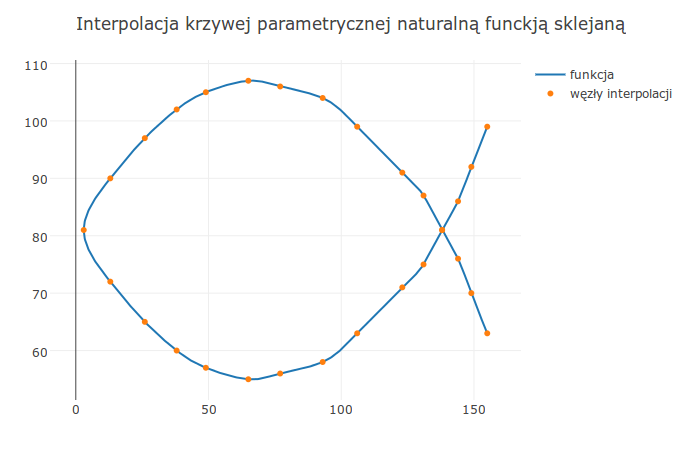
\includegraphics[width=0.8\textwidth]{newplot(2).png}
		\caption{Wykres przedstawiający rybę interpolowaną jako krzywą parametryczną naturalną funkcją sklejaną.}
		\label{Wykres:Ryba_Sklejna}
	\end{figure}
	
	Widzimy, że obrazek został odtworzony jeszcze dokładniej, niż przy metodzie \ref{podzialFunkcji} interpolowania pary funkcji.
	
	 
	
	\subsubsection{Mapa Polski}
	
	Na poniższym wykresie \ref{Wykres:Polska} przedstawiono interpolowany kontur Polski. Węzły pochodzą z listy zadań na pracownie z Analizy Numerycznej M. 
	
	\newpage
	
		\begin{figure}[h]
			\centering
			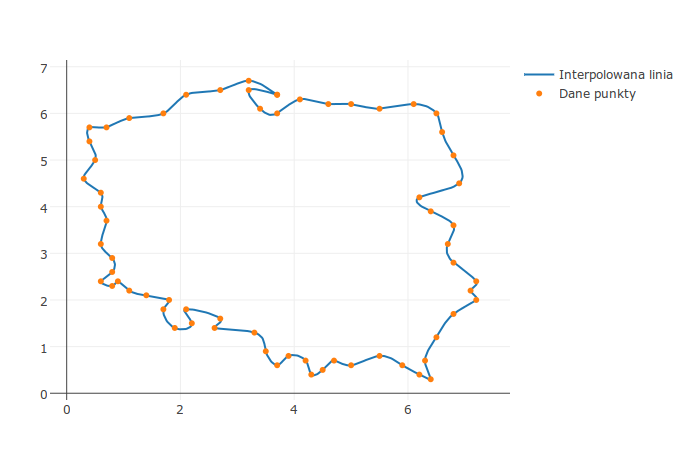
\includegraphics[width=0.8\textwidth]{newplot(3).png}
			\caption{Wykres przedstawiający interpolowany kontur Polski.}
			\label{Wykres:Polska}
		\end{figure}

	Kontur ten, jest krzywą zamkniętą, dlatego też należałoby interpolować go okresową funkcją sklejaną zamiast naturalną. Efektem niezastosowania odpowiedniej metody jest ostry kant na końcu Półwyspu Helskiego.
	
	\subsection{Krzywe parametryczne}
	
	Dotychczas z czytywaliśmy z kartki punkty, i za ich pomocą próbowaliśmy odtworzyć zadane linie. W związku tym, jedyną możliwością było subiektywne stwierdzenie, czy przybliżona linia jest ładna czy brzydka. Dlatego teraz przytoczymy parę przykładów przybliżania matematycznych krzywych parametrycznych zadanych konkretnymi wzorami. Dzięki temu, będziemy mogli policzyć normę:
	$$\sqrt{|fx(t) - Sx(t)|^2 + |fy(t) - Sx(t)|^2} $$
	
	oraz narysować wykresy błędów dla funkcji $|fx(t) - Sx(t)|$ i $|fy(t) - Sx(t)|$. Pokaże nam to faktyczną dokładność przybliżenia.
	\\\\
	Do wszystkich przykładów użyto naturalnej funkcji sklejanej trzeciego stopnia.
	
	W poniższych przykładach, sami będziemy wybierać węzły interpolacji. Warto zastanowić się nad sposobem ich rozłożenia, dlatego też przytoczmy zawężone twierdzenie zawarte w \cite{SLE}.
	
	\begin{twr} \label{tw: blad sklejanej}
		Niech $s$ będzie naturalną funkcją sklejaną III stopnia interpolującą funkcję $f \in C^2[a,b] $ w węzłach $x_0,x_1,\dots,x_n \quad (a = x_0 < x_1 < \dots < x_n = b, n \in \textbf{N} )$. Wówczas
		$$ \max_{a \leq x \leq b} |f(x) - s(x)|\leq C h^{4} \max_{a \leq x \leq b}|f(x)|, $$
		gdzie
		
		$$ C := \frac{5}{384}, \quad h := \max_{1 \leq i \leq n} h_i, \quad h_i:=x_i-x_{i-1} \quad (i = 1,2,\dots, n) $$
	\end{twr}
	
	Twierdzenie \ref{tw: blad sklejanej} pokazuje, że maksymalny błąd interpolacji zależy od stałych oraz maksymalnej odległości pomiędzy dwoma kolejnymi węzłami. Dlatego też, będziemy zawsze rozmieszczać je równomiernie. Jedynym sposobem, na zmniejszenie błędu interpolacji jest zwiększenie liczby węzłów.
	Poniższe linie interpolowano czterdziestoma węzłami interpolacji.
	
	
	\subsubsection{Spirala} 
	Krzywa parametryczna zbudowana z punktów: $(t\cos(t), t\sin(t) )$, dla $t= 0,\dots,10\pi$
	
	\begin{figure}[h]
	\centering
		\begin{subfigure}{.44\textwidth}
			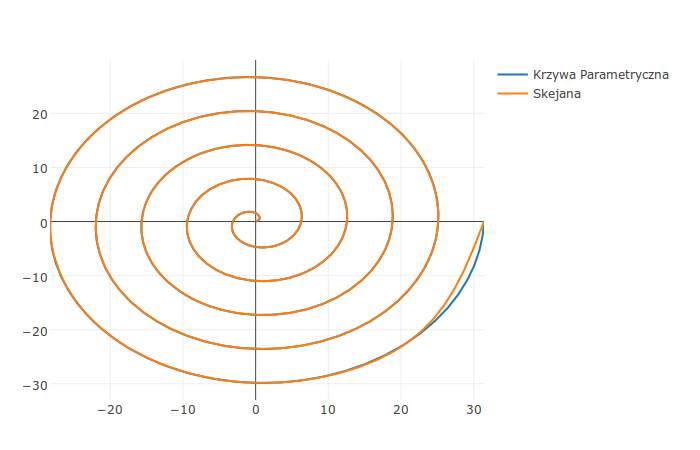
\includegraphics[width=\textwidth]{newplot(4).png}
			\caption{Krzywa parametryczna: Spirala}
			\label{Wykres:Spirala}
		\end{subfigure}
		\begin{subfigure}{.44\textwidth}
			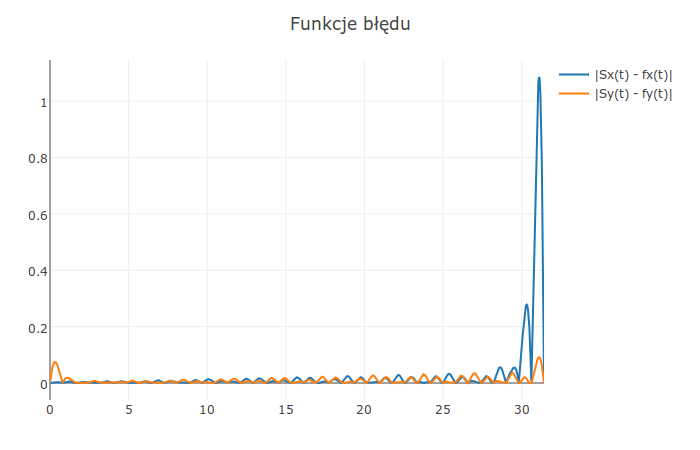
\includegraphics[width=\textwidth]{newplot(5).png}
			\caption{Błąd: Spirala}
			\label{Blad:Spirala}
		\end{subfigure}
	\end{figure}

Norma funkcji sklejanej do spirali wynosi: $1.0894$

	\subsubsection{Cykloida wydłużona}
	Krzywa parametryczna zbudowana z punktów: $(
\frac{1}{3}t-\sin(t), \frac{1}{3}-\cos(t) )$, dla $t= -3\pi,\dots,3\pi$
	\begin{figure}[h]
		\centering
		\begin{subfigure}{.44\textwidth}
			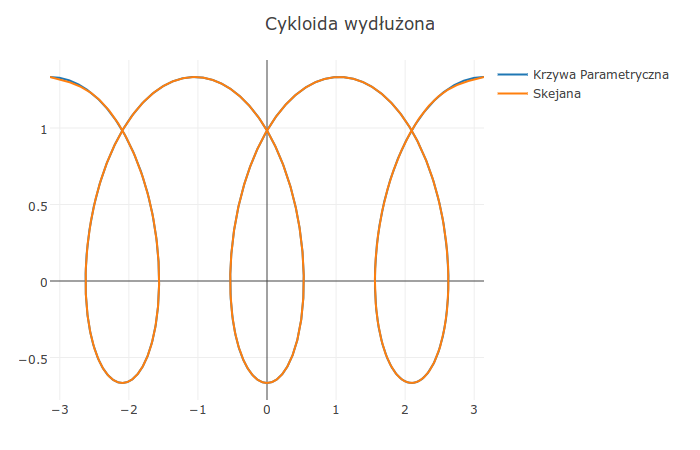
\includegraphics[width=\textwidth]{newplot(6).png}
			\caption{Krzywa parametryczna: Cykloida wydłużona}
			\label{Wykres:Cykloida}
		\end{subfigure}
		\begin{subfigure}{.44\textwidth}
			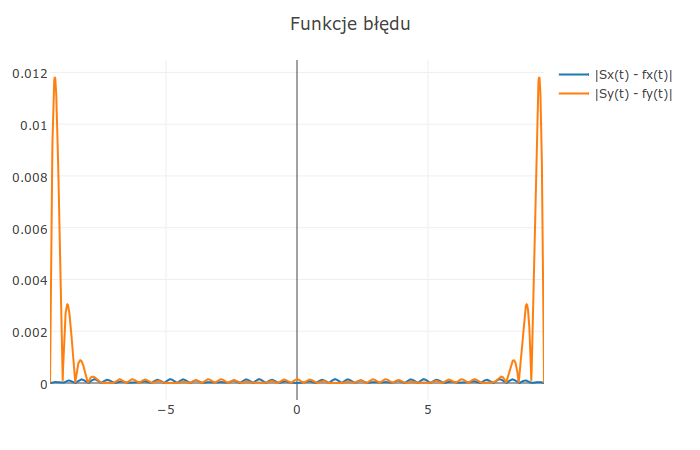
\includegraphics[width=\textwidth]{newplot(7).png}
			\caption{Błąd: Cykloida wydłużona}
			\label{Blad:Cykloida}
		\end{subfigure}
	\end{figure}

Norma funkcji sklejanej do cykloidy wynosi: $0.0118$


	\subsubsection{Krzywa z pętlami}
	Krzywa parametryczna zbudowana z punktów: $(
	t+\sin(2t), t+\sin(3t) )$, dla $t= -2\pi,\dots,2\pi$
	\begin{figure}[h]
		\centering
		\begin{subfigure}{.44\textwidth}
			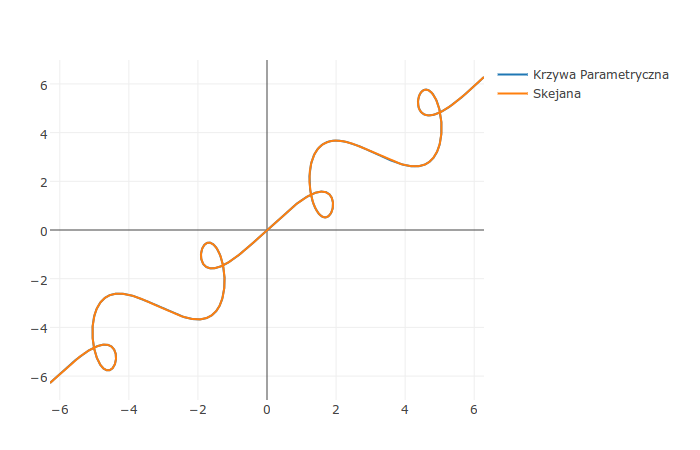
\includegraphics[width=\textwidth]{newplot(8).png}
			\caption{Krzywa parametryczna: Krzywa z pętlami}
			\label{Wykres:Krzywa z petlami}
		\end{subfigure}
		\begin{subfigure}{.44\textwidth}
			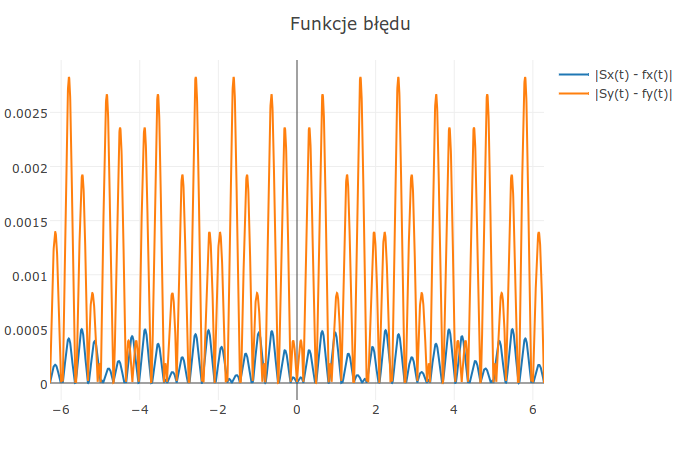
\includegraphics[width=\textwidth]{newplot(9).png}
			\caption{Błąd: Krzywa z pętlami}
			\label{Blad:Krzywa z petlami}
		\end{subfigure}
	\end{figure}
	
	Norma funkcji sklejanej do krzywej wynosi: $0.0028$
	
	\subsubsection{Globus}
		Krzywa parametryczna zbudowana z punktów: $(t\cos(t), \sin(t) )$, dla $t= 0,\dots,9\pi$
		\begin{figure}[h]
			\centering
			\begin{subfigure}{.44\textwidth}
				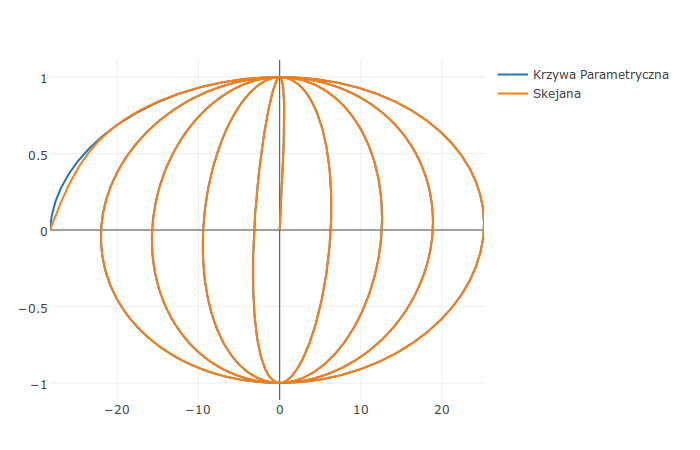
\includegraphics[width=\textwidth]{newplot(10).png}
				\caption{Krzywa parametryczna: Globus}
				\label{Wykres:Globus}
			\end{subfigure}
			\begin{subfigure}{.44\textwidth}
				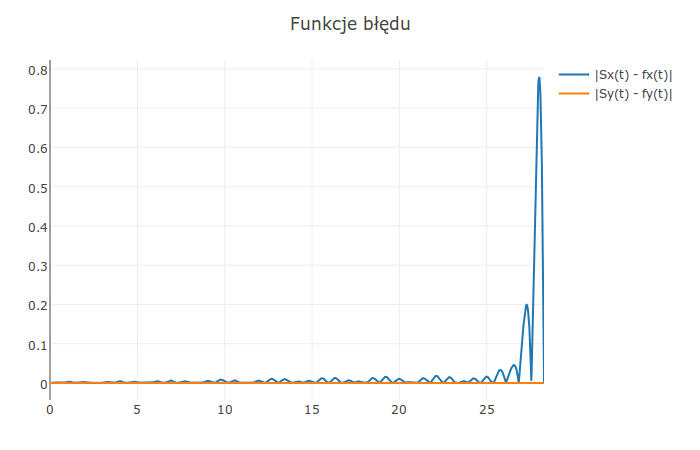
\includegraphics[width=\textwidth]{newplot(11).png}
				\caption{Błąd: Globus}
				\label{Blad:Globus}
			\end{subfigure}
		\end{figure}
		
		Norma funkcji sklejanej do globusa wynosi: $0.7793$
		

\section{Wnioski}

Interpolacja wielomianem Lagrange'a nie nadaje się do przybliżania linii, ponieważ potrafi osiągać duże błędy dla krańców przedziału.

Dzielenie linii ręcznie na poszczególne funkcję, nie nadaję się dla dużych danych.

Jedynym sposobem na zmniejszenie błędu interpolacji naturalną funkcją sklejaną III stopnia jest zwiększenie liczby węzłów interpolacji.

Interpolacja funkcji krzywej parametrycznej jest najlepszym sposobem (z podanych w sprawozdaniu) na odtworzenie w przybliżeniu linii przechodzącej przez podane punkty.







\begin{thebibliography}{9}
	\itemsep2pt
	\bibitem{kincaid} David Kincaid, Ward Cheney, przekł.~Stefan Paszkowski,
	\emph{Analiza numeryczna},
	Warszawa, WNT, 2006.
	
	\bibitem{SLE} S. Lewanowicz, {\it Analiza Numeryczna - Notatki z wykładu}, Wrocław 2007.
		
\end{thebibliography}

\end{document}
